\begin{figure}[t]
\centering
\begin{tikzpicture}[
    >=stealth,
    node distance=1.4cm and 1.8cm,
    event/.style={draw=none, font=\small},
    rf/.style={->, thick, dashed, green!60!black},
    co/.style={->, thick, dotted, red!80!black},
    ->, thick
]

% First row: G1 to G4
\begin{scope}[xshift=0cm, yshift=0cm]
  \node[event] (g1i) {init};
  \node[event, below=0.7cm of g1i] (g1r1) {$R(x)$};
  \draw[->] (g1i) -- node[midway, left] {$t_1$} (g1r1);
  \draw[rf] (g1i) to[bend left=7] (g1r1);
  \node[below=1.2cm of g1i] {(G1)};
\end{scope}

\begin{scope}[xshift=3cm, yshift=0cm]
  \node[event] (g2i) {init};
  \node[event, below=0.7cm of g2i, xshift=-0.9cm] (g2r1) {$R(x)$};
  \node[event, below=0.7cm of g2i] (g2w2) {$W(x)$};
  \draw[->] (g2i) -- node[midway, left] {$t_1$}(g2r1);
  \draw[->] (g2i) -- node[midway, right] {$t_2$}(g2w2);
  \draw[rf] (g2i) to[bend left=7] (g2r1);
  \node[below=1.2cm of g2i] {(G2)};
\end{scope}

\begin{scope}[xshift=6cm, yshift=0cm]
  \node[event] (g3i) {init};
  \node[event, below=0.7cm of g3i, xshift=-1.0cm] (g3r1) {$R(x)$};
  \node[event, below=0.7cm of g3i] (g3w2) {$W(x)$};
  \node[event, below=0.7cm of g3i, xshift=1.0cm] (g3w3) {$W(x)$};
  \draw[->] (g3i) -- node[midway, left] {$t_1$}(g3r1);
  \draw[->] (g3i) -- node[midway, right] {$t_2$}(g3w2);
  \draw[->] (g3i) -- node[midway, right, xshift=0.3cm] {$t_3$}(g3w3);
  \draw[rf] (g3i) to[bend left=10] (g3r1);
  \draw[co] (g3w2) -- (g3w3);
  \node[below=1.2cm of g3i] {(G3)};
\end{scope}

\begin{scope}[xshift=9cm, yshift=0cm]
  \node[event] (g4i) {init};
  \node[event, below=0.7cm of g4i, xshift=-1.0cm] (g4r1) {$R(x)$};
  \node[event, below=0.7cm of g4i] (g4w2) {$W(x)$};
  \node[event, below=0.7cm of g4i, xshift=1.0cm] (g4w3) {$W(x)$};
  \draw[->] (g4i) -- node[midway, left] {$t_1$}(g4r1);
  \draw[->] (g4i) -- node[midway, right] {$t_2$}(g4w2);
  \draw[->] (g4i) -- node[midway, right, xshift=0.3cm] {$t_3$}(g4w3);
  \draw[rf] (g4i) to[bend left=10] (g4r1);
  \draw[co] (g4w3) -- (g4w2);
  \node[below=1.2cm of g4i] {(G4)};
\end{scope}



% Second row: G5 to G8
\begin{scope}[xshift=0cm, yshift=-2.5cm]
  \node[event] (g5i) {init};
  \node[event, below=0.7cm of g5i, xshift=-1.0cm] (g5r1) {$R(x)$};
  \node[event, below=0.7cm of g5i, xshift=1.0cm] (g5w3) {$W(x)$};
  \draw[->] (g5i) -- node[midway, left] {$t_1$}(g5r1);
  \draw[->] (g5i) -- node[midway, right, xshift=0.3cm] {$t_3$}(g5w3);
  \draw[rf] (g5w3) to[bend left=10] (g5r1);
  \node[below=1.2cm of g5i] {(G5)};
\end{scope}

\begin{scope}[xshift=3cm, yshift=-2.5cm]
  \node[event] (g6i) {init};
  \node[event, below=0.7cm of g6i, xshift=-1.0cm] (g6r1) {$R(x)$};
  \node[event, below=0.7cm of g6i] (g6w2) {$W(x)$};
  \node[event, below=0.7cm of g6i, xshift=1.0cm] (g6w3) {$W(x)$};
  \draw[->] (g6i) -- node[midway, left] {$t_1$}(g6r1);
  \draw[->] (g6i) -- node[midway, right] {$t_2$}(g6w2);
  \draw[->] (g6i) -- node[midway, right, xshift=0.3cm] {$t_3$}(g6w3);
  \draw[rf] (g6w3) to[bend left=10] (g6r1);
  \draw[co] (g6w2) -- (g6w3);
  \node[below=1.2cm of g6i] {(G6)};
\end{scope}

\begin{scope}[xshift=6cm, yshift=-2.5cm]
  \node[event] (g7i) {init};
  \node[event, below=0.7cm of g7i, xshift=-1.0cm] (g7r1) {$R(x)$};
  \node[event, below=0.7cm of g7i] (g7w2) {$W(x)$};
  \node[event, below=0.7cm of g7i, xshift=1.0cm] (g7w3) {$W(x)$};
  \draw[->] (g7i) -- node[midway, left] {$t_1$}(g7r1);
  \draw[->] (g7i) -- node[midway, right] {$t_2$}(g7w2);
  \draw[->] (g7i) -- node[midway, right, xshift=0.3cm] {$t_3$}(g7w3);
  \draw[rf] (g7w3) to[bend left=10] (g7r1);
  \draw[co] (g7w3) -- (g7w2);
  \node[below=1.2cm of g7i] {(G7)};
\end{scope}

\begin{scope}[xshift=9cm, yshift=-2.5cm]
  \node[event] (g8i) {init};
  \node[event, below=0.7cm of g8i, xshift=-1.0cm] (g8r1) {$R(x)$};
  \node[event, below=0.7cm of g8i] (g8w2) {$W(x)$};
  \draw[->] (g8i) -- node[midway, left] {$t_1$}(g8r1);
  \draw[->] (g8i) -- node[midway, right] {$t_2$}(g8w2);
  \draw[rf] (g8w2) to[bend left=10] (g8r1);
  \node[below=1.2cm of g8i] {(G8)};
\end{scope}

% Second row: G9 to G10
\begin{scope}[xshift=0cm, yshift=-5cm]
  \node[event] (g9i) {init};
  \node[event, below=0.7cm of g9i, xshift=-1.0cm] (g9r1) {$R(x)$};
  \node[event, below=0.7cm of g9i] (g9w2) {$W(x)$};
  \node[event, below=0.7cm of g9i, xshift=1.0cm] (g9w3) {$W(x)$};
  \draw[->] (g9i) -- node[midway, left] {$t_1$}(g9r1);
  \draw[->] (g9i) -- node[midway, right] {$t_2$}(g9w2);
  \draw[->] (g9i) -- node[midway, right, xshift=0.3cm] {$t_3$}(g9w3);
  \draw[rf] (g9w2) to[bend left=10] (g9r1);
  \draw[co] (g9w2) -- (g9w3);
  \node[below=1.2cm of g9i] {(G9)};
\end{scope}

\begin{scope}[xshift=3cm, yshift=-5cm]
  \node[event] (g10i) {init};
  \node[event, below=0.7cm of g10i, xshift=-1.0cm] (g10r1) {$R(x)$};
  \node[event, below=0.7cm of g10i] (g10w2) {$W(x)$};
  \node[event, below=0.7cm of g10i, xshift=1.0cm] (g10w3) {$W(x)$};
  \draw[->] (g10i) -- node[midway, left] {$t_1$}(g10r1);
  \draw[->] (g10i) -- node[midway, right] {$t_2$}(g10w2);
  \draw[->] (g10i) -- node[midway, right, xshift=0.3cm] {$t_3$}(g10w3);
  \draw[rf] (g10w2) to[bend left=10] (g10r1);
  \draw[co] (g10w3) -- (g10w2);
  \node[below=1.2cm of g10i] {(G10)};
\end{scope}

\end{tikzpicture}
\caption{Execution graphs illustrating different read-from and coherence orders among three threads.}
\label{exec-graphs}
\end{figure}


\begin{figure}[h]
\centering
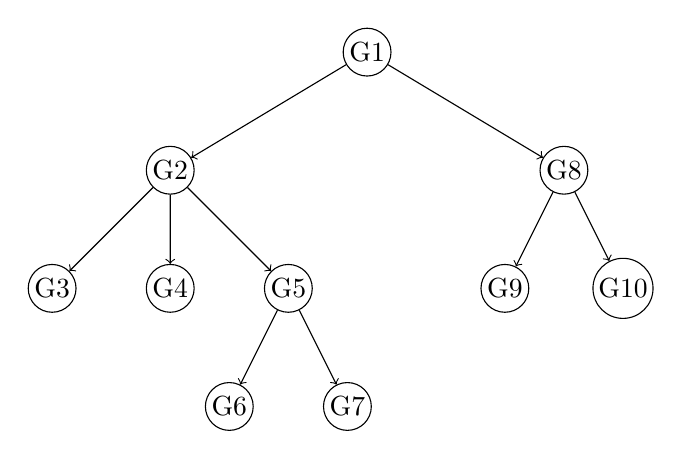
\begin{tikzpicture}[
  level distance=1.5cm,
  sibling distance=1.5cm,
  edge from parent/.style={->, draw},
  every node/.style={circle, draw, minimum size=6mm, inner sep=1pt},
  level 1/.style={sibling distance=5cm},
  level 2/.style={sibling distance=1.5cm}
  ]

\node (G1) {G1}
  child {node (G2) {G2}
    child {node (G3) {G3}}
    child {node (G4) {G4}}
    child {node (G5) {G5}
        child {node (G6) {G6}}
        child {node (G7) {G7}}
        }
  }
  child {node (G8) {G8}
    child {node (G9) {G9}}
    child {node (G10) {G10}}
  };

\end{tikzpicture}
\caption{backtracking tree tree of Trust over execution graphs.}
\label{fig:graph-tree}
\end{figure}
